\documentclass[tikz,border=6mm]{standalone}
\usepackage{tikz}
\usepackage{xcolor}
\usetikzlibrary{arrows.meta,calc,decorations.pathmorphing,shapes.geometric,positioning,backgrounds,fit,shadings,patterns}
\definecolor{substblue}{RGB}{70,130,180}
\definecolor{procamber}{RGB}{180,110,30}
\definecolor{feltgreen}{RGB}{0,110,55}
\definecolor{bgcream}{RGB}{252,248,240}
\definecolor{atomblue}{RGB}{100,160,210}
\definecolor{emphred}{RGB}{160,40,40}
\definecolor{panelborder}{RGB}{180,170,155}

\begin{document}
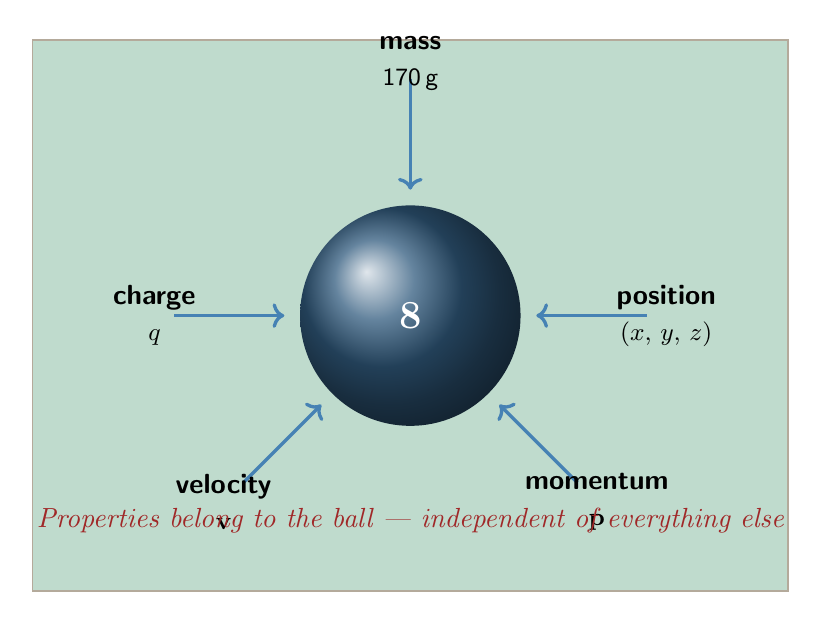
\begin{tikzpicture}[
  every node/.style={font=\sffamily},
  lbl arrow/.style={->, very thick, substblue, shorten >=2mm},
]

%% Background felt rectangle
\fill[feltgreen!25, draw=panelborder, line width=0.6pt]
  (-4.8,-3.5) rectangle (4.8,3.5);

%% Billiard ball with ball shading
\shade[ball color=substblue!70!black] (0,0) circle (1.4cm);

%% White "8" label on ball
\node[white, font=\bfseries\Large] at (0,0) {8};

%% ---- Arrows (from label positions toward ball edge) ----

% Top (90°): label at (0, 3.2), arrow tip at ball edge along 90°
\draw[lbl arrow] (0, 3.0) -- (0, 1.4);
\node[align=center] at (0, 3.2)
  {\textbf{mass}\\[1pt]\small 170\,g};

% Right (0°): label at (3.2, 0)
\draw[lbl arrow] (3.0, 0) -- (1.4, 0);
\node[align=center] at (3.25, 0)
  {\textbf{position}\\[1pt]\small $(x,\,y,\,z)$};

% Lower-right (−45°): tip at ball edge
\draw[lbl arrow]
  ({3.0*cos(-45)}, {3.0*sin(-45)}) --
  ({1.4*cos(-45)}, {1.4*sin(-45)});
\node[align=center] at ({3.35*cos(-45)}, {3.35*sin(-45)})
  {\textbf{momentum}\\[1pt]\small $\mathbf{p}$};

% Lower-left (−135°)
\draw[lbl arrow]
  ({3.0*cos(-135)}, {3.0*sin(-135)}) --
  ({1.4*cos(-135)}, {1.4*sin(-135)});
\node[align=center] at ({3.35*cos(-135)}, {3.35*sin(-135)})
  {\textbf{velocity}\\[1pt]\small $\mathbf{v}$};

% Left (180°)
\draw[lbl arrow] (-3.0, 0) -- (-1.4, 0);
\node[align=center] at (-3.25, 0)
  {\textbf{charge}\\[1pt]\small $q$};

%% Caption below ball
\node[emphred, font=\itshape, align=center] at (0,-2.6)
  {Properties belong to the ball --- independent of everything else};

\end{tikzpicture}
\end{document}
